\newpage
\section{Aufbau und Durchführung}
\subsection{Der Laser}
Das Medium des HeNe-Lasers besteht aus einem Anteil von $5:1$ aus He- und Ne-Atomen.
Dieses Gasgemische, was das Lasermedium bildet, befindet sich in einem Laserrohr mit einem Druck von 1 Torr. Die Besetzunginversion wird durch die
elektrische Entladung erreicht. Die somit angeregten He-Atome stoßen mit den Ne-Atomen und übertragen somit ihre Energie.
Da es sich hierbei wie zuvor beschrieben um ein Mehr-Niveau-System handelt liegen auch mehrere Laserlinien vor, wobei die Wellenlänge
$\lambda=632,8$nm am ausgeprägtesten/intensivsten ist.\\
\begin{figure}[H]
    \center
    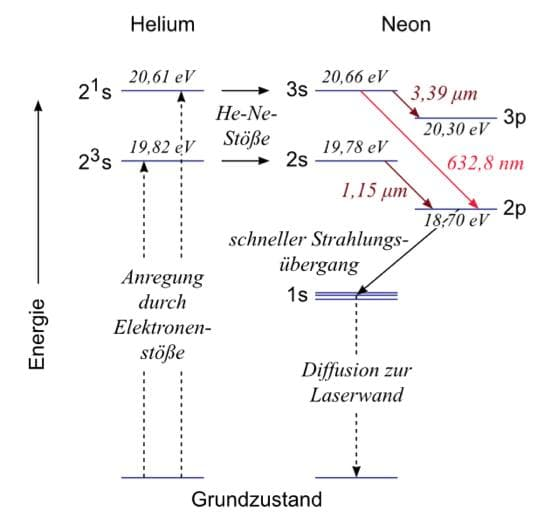
\includegraphics[width=0.7\textwidth]{bilder/lasermedium.jpg}
    \caption{Darstellung der Energiezustände des HeNe-Gasgemisches.}
\end{figure}

Um einen möglich verlustfreien Durchtritt des Lichtes in das Laserrohr zu gewährleisten, ist das Rohr mit Brewsterfenstern abgeschlossen.
Durch die Ausrichtung der Flächen im Brewsterwinkel zu optischen Achse wird das parralel zur Einfallsebene polarisierte Licht nicht durch Reflexionseffekte abgeschwächt.

\subsection{Der Aufbau}
Der Aufbau besteht aus einer optischen Schiene auf der sich ein Justierlaser mit den Kenngrößen $\lambda=532\,$nm und $P_{\text{red}}=0,2\,$mW, 
zwei Resonatorspiegel, ein Laserrohr und Blenden befindet. Das Laserrohr hat eine Länge von $l=408$mm und einen Duchmesser
von $d_{\text{HeNe}}=1,1$mm und ist mit dem HeNe Gasgemisch gefüllt und mit einer Elektrode verbunden.
Für den optischen Resonator stehen verschieden Spiegel zur Verfügung.
\begin{description}
    \item[konkaver Spiegel] mit $r=1400$mm und einem Tansmissionswert von $T=1,5;...1,8\%$
    \item[plamarer Spiegel] mit $r=1400$mm und einer Reflektivität von $R>99\%$
    \item[konkaver Spiegel] mit $r=1400$mm und einer Reflektivität von $R>99\%$
    \end{description}
Für die Justage kann der Justierlaser mit einem passenden Fadenkreuz verwendet werden.
\begin{figure}[H]
    \center
    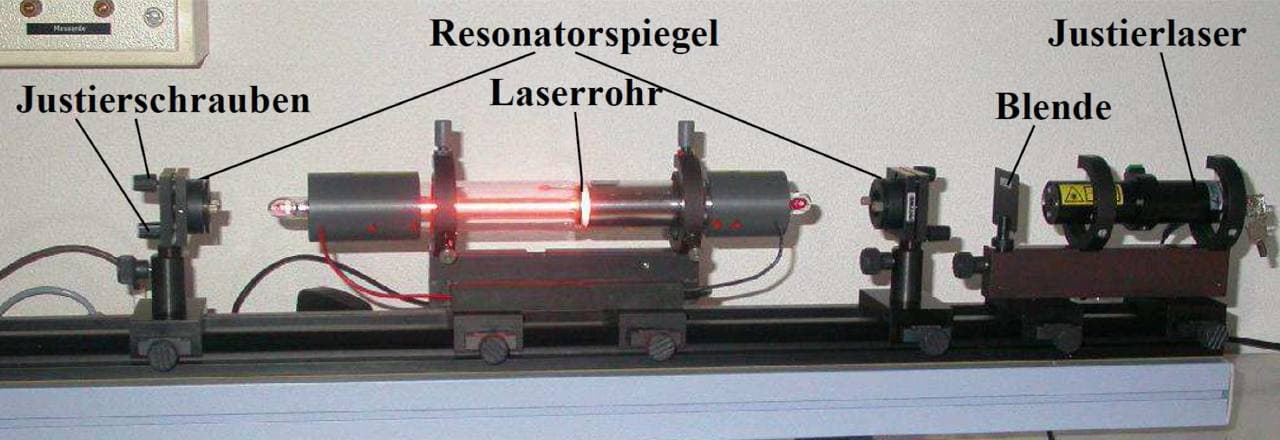
\includegraphics[width=\textwidth]{bilder/laser.jpg}
    \caption{Aufbau des HeNe-Lasers \cite{anleitung}}
\end{figure}

\subsection{Durchführung}
\subsubsection{Justage}
Der Justierlaser wird mit beiden Beugungsblenden auf die optische Schiene gestellt. Dabei haben die Blenden
einen maximalen Abstand zueinander. Der Justierlaser wird nun so ausgerichtet, dass sich das Fadenkreuz genau in der Mitte der Beugungsringe
befindet. Danach werden Resonatorspiegel und Laserrohr auf die optische Schiene hinzugefügt und der Strom der Hochspannung mit $I=6.5\,$mA eingeschaltet werden.
Um die Lasertätigkeit zu aktivieren werden nun die Spiegel nachjustiert. 
\subsubsection{Stabilitätsbedingung}
Über eine Photodiode wird die maximale Leistung des Lasers eingestellt. Fortlaufend wird nun der Abstand der Resonatorspiegel
vergrößert und die Laserleistung nachjustiert. Diese Messung wird jeweils für eine plan-konkav und konkav-konkav Spiegelkonfiguration durchgeführt.
\subsubsection{TEM-Moden}
Um die TEM-Moden zu beobachten wird ein dünner Wolframdraht der Dicke $d=0,005\,$mm verwendet. Dieser wird zwischen Lasserrohr und Resonatorspiegel gebracht.
Durch das Verschieben des Drahtes werden verschiedene Moden auf dem optischen Schirm sichtbar. Die Mode wird daraufhin mit einer Photodiode vom Zentrum ($x=0\,$mm) aus vermessen.
\subsubsection{Polarisationsbestimmung}
Mithilfe eines Polarisator der hinter den Auskopplungsspiegel positioniert wird kann mithilfe einer Photodiode die Intensität in Abhängigkeit
der jeweiligen Polarisationsrichtung vermessen werden und somit die Polarisation des Lasers bestimmt werden.

\label{sec:Durchfuehrung}
